%
% hardware.tex
%
% Copyright The TTC 2.0 Contributors.
%
% TTC 2.0 Documentation
%
% This work is licensed under the Creative Commons Attribution-ShareAlike 4.0
% International License. To view a copy of this license,
% visit http://creativecommons.org/licenses/by-sa/4.0/.
%

%
% \brief Hardware project chapter.
%
% \author Gabriel Mariano Marcelino <gabriel.mm8@gmail.com>
%
% \version 0.3.0
%
% \date 2021/04/02
%


\chapter{Hardware} \label{ch:hardware}

This chapter presents a description of the hardware project of the TTC 2.0 module. As the primary reference, a block diagram can be seen in \autoref{fig:hardware-diagram}. Also, a 3D model of both sides of the PCB is available in \autoref{fig:ttc2-3d-surface}.

\begin{figure}[!ht]
	\begin{center}
		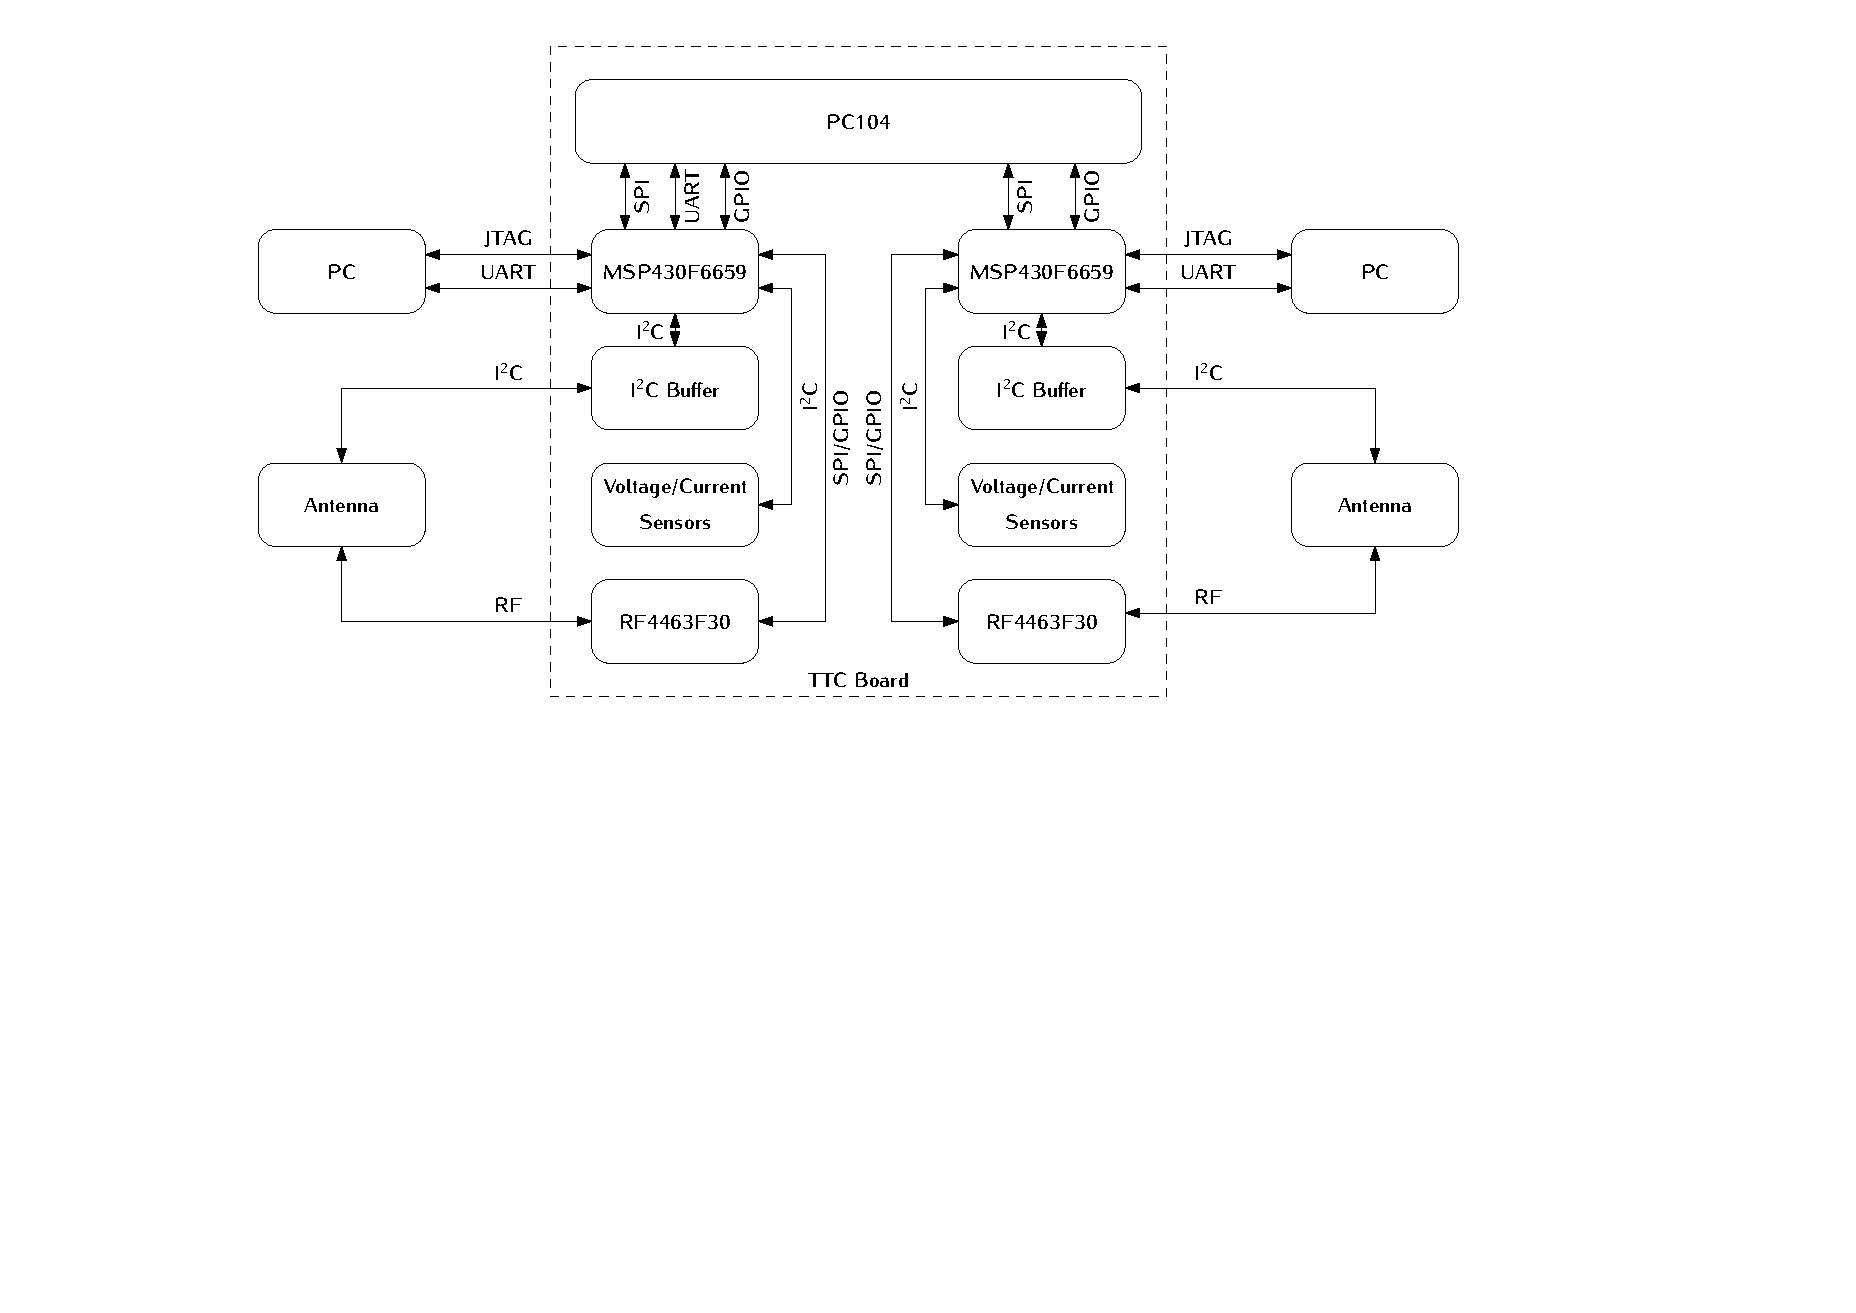
\includegraphics[width=\textwidth]{figures/hardware_diagram.pdf}
		\caption{Block diagram of the TTC 2.0 hardware.}
		\label{fig:hardware-diagram}
	\end{center}
\end{figure}

\begin{figure}[!ht]
    \begin{center}
        \subfigure[Upper surface of the TTC 2.0 PCB.\label{fig:ttc2-pcb-top}]{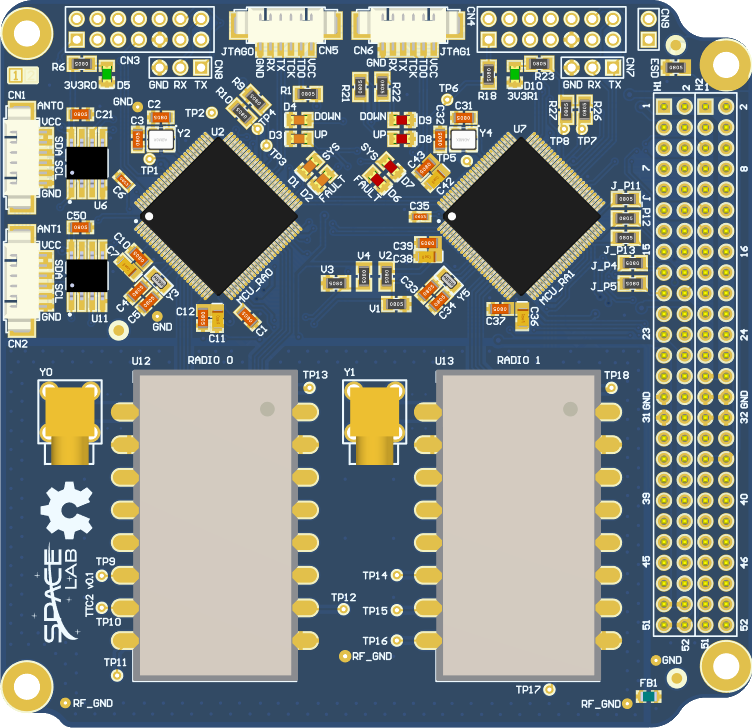
\includegraphics[width=0.48\textwidth]{figures/ttc2_pcb_top}}
        ~
        \subfigure[Lower surface of the TTC 2.0 PCB.\label{fig:ttc2-pcb-bottom}]{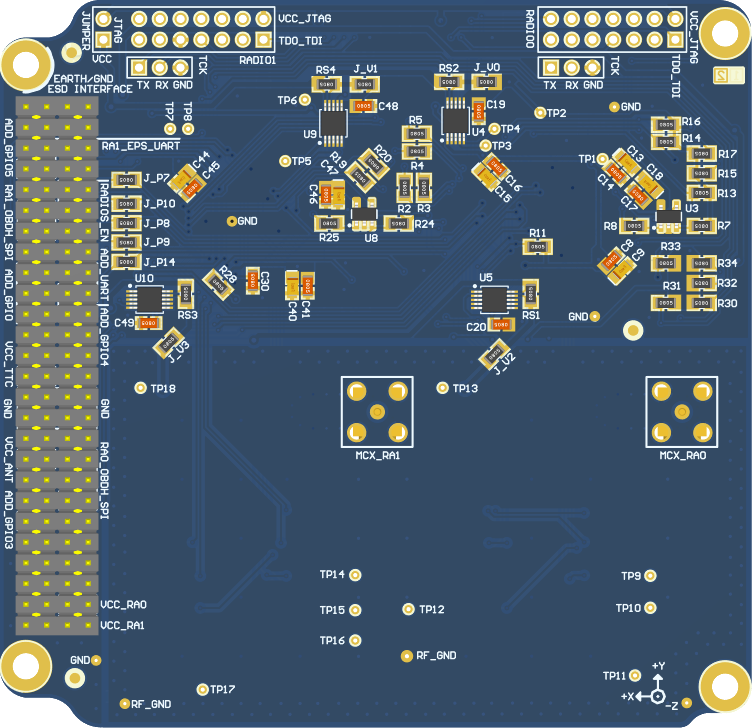
\includegraphics[width=0.48\textwidth]{figures/ttc2_pcb_bottom}}
        \caption{Surfaces of the 3D model of the TTC 2.0 board.}
        \label{fig:ttc2-3d-surface}
    \end{center}
\end{figure}

The following sections present a further description of the hardware project.

\section{Specifications}

The TTC 2.0 has two microcontrollers (MSP430FR6659) that run at a clock of 32 MHz, a RAM of 64 kB (SRAM), a flash memory of 512 kB for code storage, and another one of 128 kB for data storage. The TTC 2.0 also has current, voltage, and temperature sensors and two radio modules for RF communication. A brief description of the general specifications of the TTC 2.0 module is available below:

\begin{itemize}
    \item \textbf{Microcontroller}: MSP430F6659
    \item \textbf{Clock}: 32 MHz
    \item \textbf{Memories}:
    \begin{itemize}
        \item RAM: 64 kB (SRAM)
        \item Flash: 512 kB (code) and 128 kB (storage)
    \end{itemize}
    \item \textbf{Sensors}: Voltage, current and temperature
    \item \textbf{Modulation}: (G)FSK and/or (G)MSK
    \item \textbf{Baudrate}: 1200 to 9600 bps
    \item \textbf{Frequency}: 145-146 MHz, 435-438 MHz, and/or 450 MHz bands
    \item \textbf{Protocol}: NGHam
    \item \textbf{Interfaces}: UART, I$^{2}$C and SPI
    \item \textbf{Mass}: 73 g
    \item \textbf{Main bus}: PC-104 standard
\end{itemize}

\section{Electrical interfaces}

Below is a description of all available electrical interfaces of the TTC 2.0 module. The interfaces can be divided into PC-104 bus and dedicated interfaces.

\subsection{PC-104 bus}

The connector PC-104 is a junction of two double rows 26 pin headers (\textit{SSW-126-04-G-D} by default). These connectors create a solid 104-pin interconnection across the different satellite modules. \autoref{tab:pc104-pinout} provides the connector pinout\footnote{This pinout is simplified since additional interfaces were omitted.} for the pins that are connected to the module. A reference of the pin's position can also be seen in \autoref{fig:pc104-ref-diagram}, and a description of the signal is available in \autoref{tab:pc104-signals}.

\begin{figure}[!ht]
    \begin{center}
        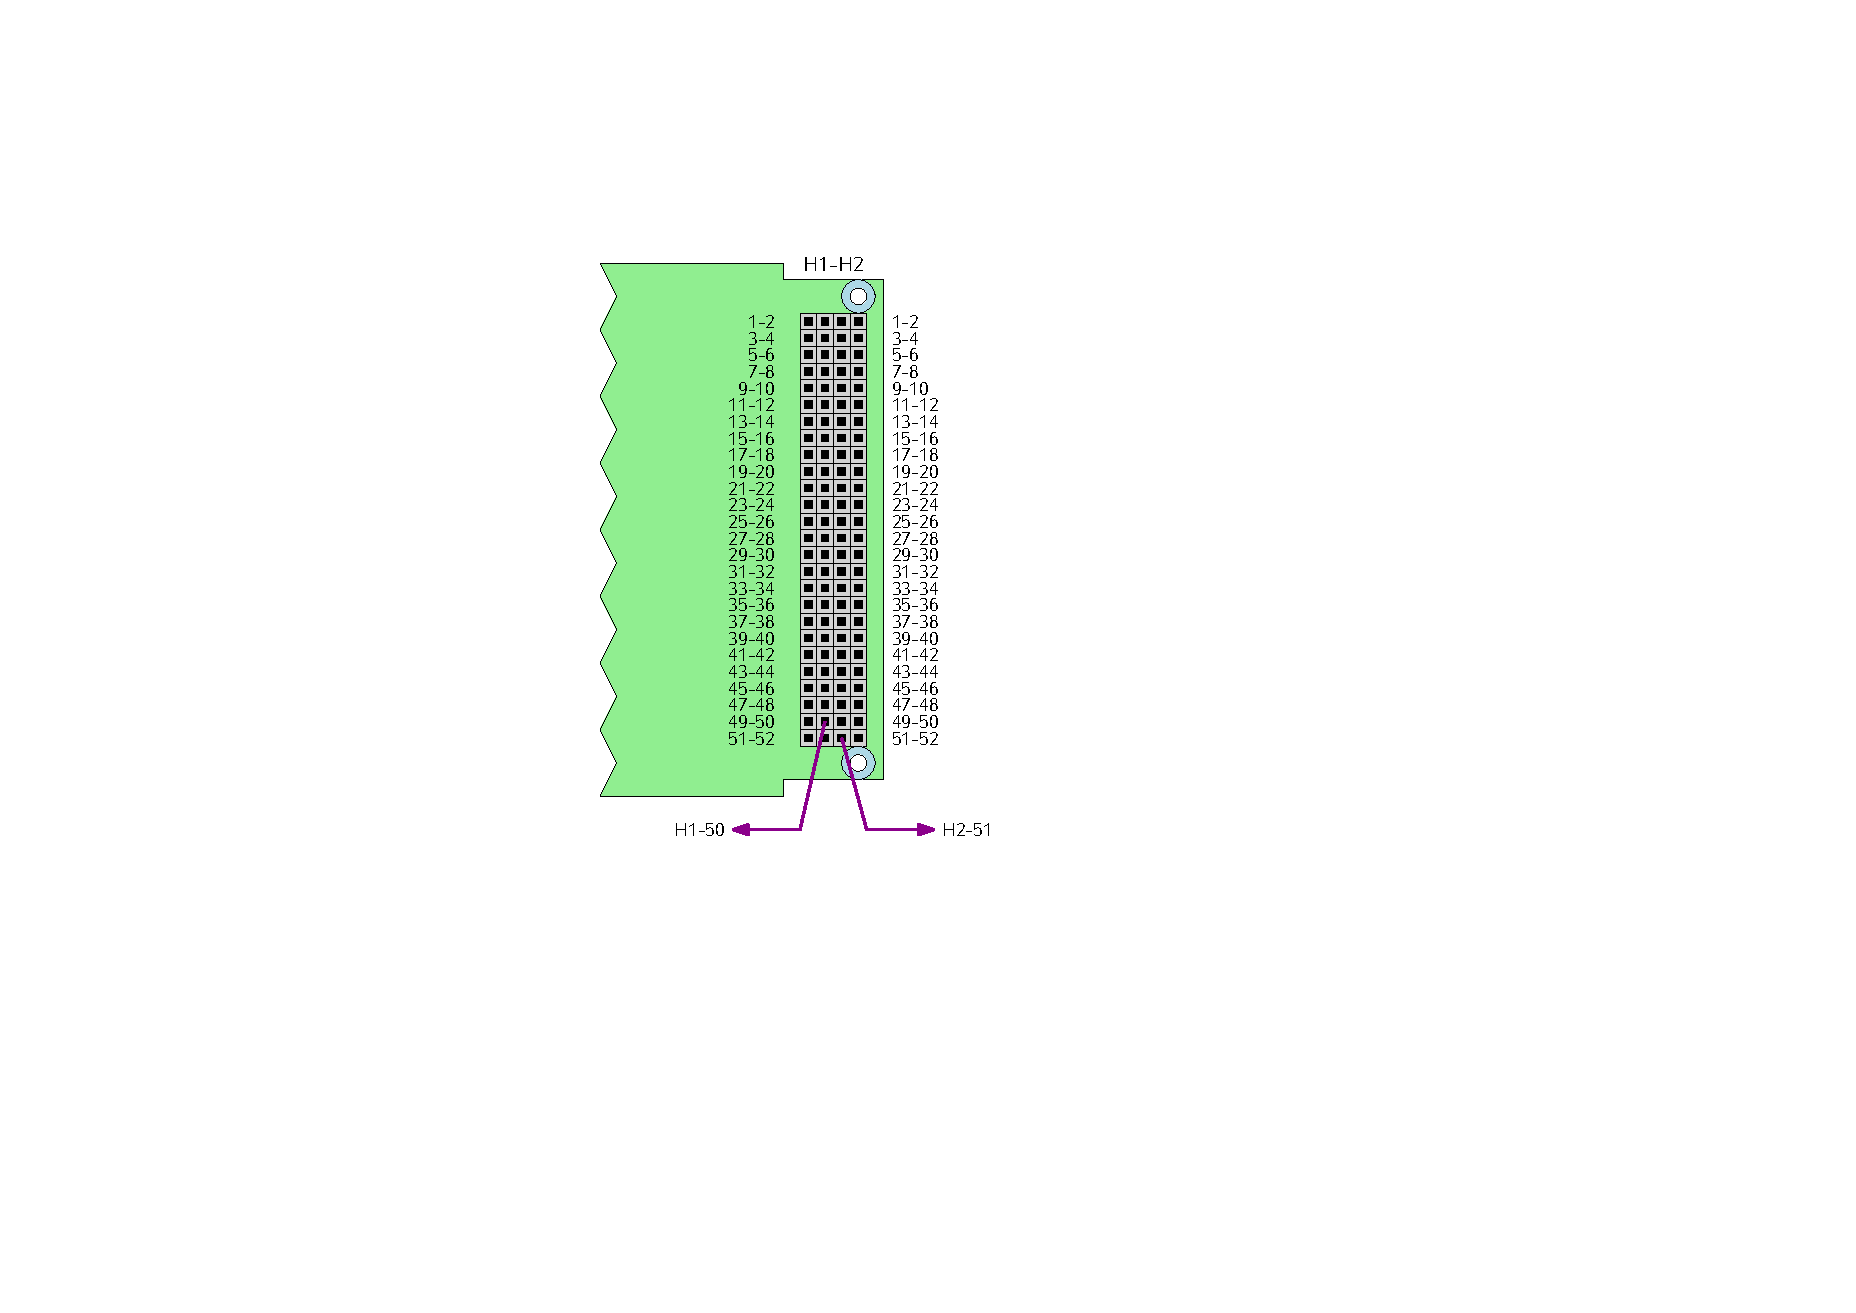
\includegraphics[width=0.5\textwidth]{figures/pc104-diagram}
        \caption{Reference diagram of the PC-104 bus (top view of a generic module).}
        \label{fig:pc104-ref-diagram}
    \end{center}
\end{figure}

\begin{table}[!ht]
    \centering
    \begin{tabular}{cllll}
        \toprule[1.5pt]
        \textbf{Pin Row}   & \textbf{H1 Odd}  & \textbf{H1 Even} & \textbf{H2 Odd}  & \textbf{H2 Even} \\
        \midrule
        1-2                & -                & -                & -                & -                \\
        3-4                & -                & -                & -                & -                \\
        5-6                & -                & -                & RA\_1\_UART\_RX  & -                \\
        7-8                & GPIO\_6          & GPIO\_7          & RA\_1\_UART\_TX  & GPIO\_0          \\
        9-10               & RA\_1\_SPI\_INT  & RA\_1\_EN        & -                & -                \\
        11-12              & RA\_0\_SPI\_INT  & RA\_0\_EN        & RA\_1\_SPI\_MOSI & RA\_1\_SPI\_CLK  \\
        13-14              & -                & -                & RA\_1\_SPI\_CS   & RA\_1\_SPI\_MISO \\
        15-16              & -                & -                & -                & -                \\
        17-18              & -                & -                & -                & GPIO\_1          \\
        19-20              & -                & GPIO\_2          & -                & GPIO\_3          \\
        21-22              & -                & -                & -                & GPIO\_4          \\
        23-24              & -                & -                & -                & -                \\
        25-26              & -                & -                & -                & -                \\
        27-28              & -                & -                & VCC\_3V3         & VCC\_3V3         \\
        29-30              & GND              & GND              & GND              & GND              \\
        31-32              & GND              & GND              & GND              & GND              \\
        33-34              & -                & -                & -                & -                \\
        35-36              & RA\_0\_SPI\_CLK  & -                & VCC\_3V3\_ANT    & VCC\_3V3\_ANT    \\
        37-38              & RA\_0\_SPI\_MISO & -                & -                & -                \\
        39-40              & RA\_0\_SPI\_MOSI & RA\_0\_SPI\_CS   & -                & -                \\
        41-42              & -                & -                & -                & GPIO\_5          \\
        43-44              & -                & -                & -                & -                \\
        45-46              & -                & -                & -                & -                \\
        47-48              & -                & -                & -                & -                \\
        49-50              & VCC\_5V\_RA\_0   & VCC\_5V\_RA\_0   & -                & -                \\
        51-52              & VCC\_6V\_RA\_1   & VCC\_6V\_RA\_1   & -                & -                \\
        \bottomrule[1.5pt]
    \end{tabular}
    \caption{PC-104 bus pinout.}
    \label{tab:pc104-pinout}
\end{table}

\begin{table}[!ht]
    \centering
    \begin{tabular}{lL{0.3\textwidth}l}
        \toprule[1.5pt]
        \textbf{Signal}  & \textbf{Pin(s)}                  & \textbf{Description} \\
        \midrule
        GND              & H1-29/30/31/32, H2-29/30/31/32   & Ground reference                      \\
        VCC\_3V3         & H2-27, H2-28                     & TTC power supply (3,3 V)              \\
        VCC\_3V3\_ANT    & H2-35, H2-36                     & Antenna power supply (3,3 V)          \\
        VCC\_5V\_RA\_0   & H1-49, H1-50                     & Radio 0 power supply (5 V)            \\
        VCC\_6V\_RA\_1   & H1-51, H1-52                     & Radio 1 power supply (6 V)            \\
        RA\_0\_SPI\_CLK  & H1-35                            & CLK signal of the radio 0 SPI bus     \\
        RA\_0\_SPI\_MISO & H1-37                            & MISO signal of the radio 0 SPI bus    \\
        RA\_0\_SPI\_MOSI & H1-39                            & MOSI signal of the radio 0 SPI bus    \\
        RA\_0\_SPI\_CS   & H1-40                            & CS signal of the radio 0 SPI bus      \\
        RA\_0\_SPI\_INT  & H1-11                            & INT signal of the radio 0 SPI bus     \\
        RA\_1\_SPI\_CLK  & H2-12                            & CLK signal of the radio 0 SPI bus     \\
        RA\_1\_SPI\_MISO & H2-14                            & MISO signal of the radio 0 SPI bus    \\
        RA\_1\_SPI\_MOSI & H2-11                            & MOSI signal of the radio 0 SPI bus    \\
        RA\_1\_SPI\_CS   & H1-13                            & CS signal of the radio 0 SPI bus      \\
        RA\_1\_SPI\_INT  & H1-9                             & INT signal of the radio 0 SPI bus     \\
        RA\_1\_UART\_RX  & H2-5                             & RX signal of the radio 1 UART         \\
        RA\_1\_UART\_TX  & H2-7                             & TX signal of the radio 1 UART         \\
        RA\_0\_EN        & H1-11                            & Radio 0 power enable                  \\
        RA\_1\_EN        & H1-9                             & Radio 1 power enable                  \\
        GPIO\_N          & H1-7/8/19, H2-8/18/20/22/42      & GPIO pin (not used)                   \\
        \bottomrule[1.5pt]
    \end{tabular}
    \caption{PC-104 bus signal description.}
    \label{tab:pc104-signals}
\end{table}

This project's distribution pattern of pins is a mix of multiple patterns from CubeSat module manufacturers, like GomSpace, ISISpace, and EnduroSat. Some pins are positioned to attend to specific project requirements; this way, it is possible that the adopted pattern is only partially compatible with some commercial modules or other custom projects.

\subsection{Dedicated electrical interfaces}

The module also contains other electrical interfaces through pin headers and PicoBlade connectors that are used to flash code and as debug port of microcontrollers (CN5, CN3, CN4, CN6) and serial communication for a status report and log messages (CN7, CN8). The C9 connector switches the TTC 2.0 power supply to the MSP-FET. The CN1 and CN2 are antenna interfaces (I$^{2}$C bus and power), and Y0, Y1 are MCX connectors to be used as the RF interface with the antennas. More details of each of these connectors, like the pinout, can be seen in \autoref{tab:icd}.

\begin{longtable}[c]{lcccl}
    \toprule[1.5pt]
    \textbf{Connector} & \textbf{Image} & \textbf{Interface} & \textbf{Type} & \textbf{Pins} \\
    \midrule
    \multirow{10}{*}{CN1} & \multirow{10}{*}{\raisebox{-\totalheight}{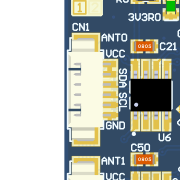
\includegraphics[width=4cm]{figures/cn1}}} & \multirow{10}{*}{I$^{2}$C} & \multirow{10}{*}{PicoBlade} &  \\
                          &  &                           &                            &  \\
                          &  &                           &                            & 3V3 \\
                          &  &                           &                            & 3V3 \\
                          &  &                           &                            & I2C\_SDA \\
                          &  &                           &                            & I2C\_SCL \\
                          &  &                           &                            & GND \\
                          &  &                           &                            & GND \\
                          &  &                           &                            &  \\
                          &  &                           &                            &  \\
    \midrule
    \multicolumn{5}{r}{\textit{Continues on next page}} \\
    \pagebreak
    \midrule
    \multirow{10}{*}{CN2} & \multirow{10}{*}{\raisebox{-\totalheight}{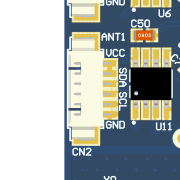
\includegraphics[width=4cm]{figures/cn2}}} & \multirow{10}{*}{I$^{2}$C} & \multirow{10}{*}{PicoBlade} &  \\
                          &  &                           &                            &  \\
                          &  &                           &                            & 3V3 \\
                          &  &                           &                            & 3V3 \\
                          &  &                           &                            & I2C\_SDA \\
                          &  &                           &                            & I2C\_SCL \\
                          &  &                           &                            & GND \\
                          &  &                           &                            & GND \\
                          &  &                           &                            & \\
                          &  &                           &                            & \\
    \midrule
    \multirow{10}{*}{CN5} & \multirow{10}{*}{\raisebox{-\totalheight}{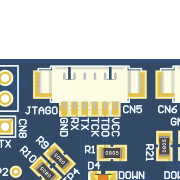
\includegraphics[width=4cm]{figures/cn5}}} & \multirow{10}{*}{JTAG} & \multirow{10}{*}{PicoBlade} &  \\
                          &  &                           &                            &  \\
                          &  &                           &                            & 3V3\_JTAG \\
                          &  &                           &                            & TDO\_TDI \\
                          &  &                           &                            & TCK \\
                          &  &                           &                            & UART\_TX \\
                          &  &                           &                            & UART\_RX \\
                          &  &                           &                            & GND \\
                          &  &                           &                            & \\
                          &  &                           &                            & \\
    \midrule
    \multirow{10}{*}{CN6} & \multirow{10}{*}{\raisebox{-\totalheight}{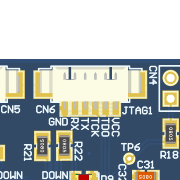
\includegraphics[width=4cm]{figures/cn6}}} & \multirow{10}{*}{JTAG} & \multirow{10}{*}{PicoBlade} &  \\
                          &  &                           &                            &  \\
                          &  &                           &                            & 3V3\_JTAG \\
                          &  &                           &                            & TDO\_TDI \\
                          &  &                           &                            & TCK \\
                          &  &                           &                            & UART\_TX \\
                          &  &                           &                            & UART\_RX \\
                          &  &                           &                            & GND \\
                          &  &                           &                            & \\
                          &  &                           &                            & \\
    \midrule
    \multirow{10}{*}{CN7} & \multirow{10}{*}{\raisebox{-\totalheight}{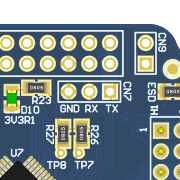
\includegraphics[width=4cm]{figures/cn7}}} & \multirow{10}{*}{UART} & \multirow{10}{*}{PinHeader} &  \\
                          &  &                           &                            &  \\
                          &  &                           &                            &  \\
                          &  &                           &                            & TX \\
                          &  &                           &                            & RX \\
                          &  &                           &                            & GND \\
                          &  &                           &                            &  \\
                          &  &                           &                            &  \\
                          &  &                           &                            &  \\
                          &  &                           &                            &  \\
    \midrule
    \multicolumn{5}{r}{\textit{Continues on next page}} \\
    \pagebreak
    \midrule
    \multirow{10}{*}{CN8} & \multirow{10}{*}{\raisebox{-\totalheight}{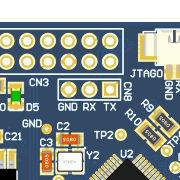
\includegraphics[width=4cm]{figures/cn8}}} & \multirow{10}{*}{UART} & \multirow{10}{*}{PicoBlade} &  \\
                          &  &                           &                            &  \\
                          &  &                           &                            &  \\
                          &  &                           &                            & TX \\
                          &  &                           &                            & RX \\
                          &  &                           &                            & GND \\
                          &  &                           &                            &  \\
                          &  &                           &                            &  \\
                          &  &                           &                            &  \\
                          &  &                           &                            &  \\
    \midrule
    \multirow{10}{*}{CN9}  & \multirow{10}{*}{\raisebox{-\totalheight}{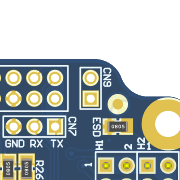
\includegraphics[width=4cm]{figures/cn9}}} & \multirow{10}{*}{Jumper} & \multirow{10}{*}{Pin Header} &  \\
                          &  &                           &                            &  \\
                          &  &                           &                            &  \\
                          &  &                           &                            &  \\
                          &  &                           &                            & 3V3\_JTAG \\
                          &  &                           &                            & 3V3 \\
                          &  &                           &                            &  \\
                          &  &                           &                            &  \\
                          &  &                           &                            &  \\
                          &  &                           &                            &  \\
    \midrule
    \multirow{14}{*}{CN3} & \multirow{14}{*}{\raisebox{-\totalheight}{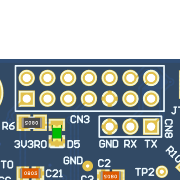
\includegraphics[width=4cm]{figures/cn3}}} & \multirow{14}{*}{JTAG} & \multirow{14}{*}{Pin Header} & TDO\_TDI \\
                          &  &                           &                            & 3V3\_JTAG \\
                          &  &                           &                            & None \\
                          &  &                           &                            & None \\
                          &  &                           &                            & None \\
                          &  &                           &                            & None \\
                          &  &                           &                            & TCK \\
                          &  &                           &                            & None \\
                          &  &                           &                            & GND \\
                          &  &                           &                            & None \\
                          &  &                           &                            & None \\
                          &  &                           &                            & UART\_TX \\
                          &  &                           &                            & None \\
                          &  &                           &                            & UART\_RX \\
    \midrule
    \multicolumn{5}{r}{\textit{Continues on next page}} \\
    \pagebreak
    \midrule
    \multirow{14}{*}{CN4} & \multirow{14}{*}{\raisebox{-\totalheight}{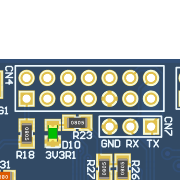
\includegraphics[width=4cm]{figures/cn4}}} & \multirow{14}{*}{JTAG} & \multirow{14}{*}{Pin Header} & TDO\_TDI \\
                          &  &                           &                            & 3V3\_JTAG \\
                          &  &                           &                            & None \\
                          &  &                           &                            & None \\
                          &  &                           &                            & None \\
                          &  &                           &                            & None \\
                          &  &                           &                            & TCK \\
                          &  &                           &                            & None \\
                          &  &                           &                            & GND \\
                          &  &                           &                            & None \\
                          &  &                           &                            & None \\
                          &  &                           &                            & UART\_TX \\
                          &  &                           &                            & None \\
                          &  &                           &                            & UART\_RX \\
    \midrule
    \multirow{10}{*}{Y0}  & \multirow{10}{*}{\raisebox{-\totalheight}{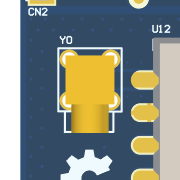
\includegraphics[width=4cm]{figures/y0}}} & \multirow{10}{*}{RF} & \multirow{10}{*}{MCX} &  \\
                          &  &                           &                            &  \\
                          &  &                           &                            &  \\
                          &  &                           &                            &  \\
                          &  &                           &                            & RF\_SIGNAL \\
                          &  &                           &                            & RF\_GND \\
                          &  &                           &                            &  \\
                          &  &                           &                            &  \\
                          &  &                           &                            &  \\
                          &  &                           &                            &  \\
    \midrule
    \multirow{10}{*}{Y1}  & \multirow{10}{*}{\raisebox{-\totalheight}{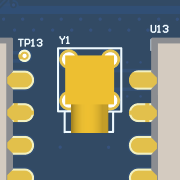
\includegraphics[width=4cm]{figures/y1}}} & \multirow{10}{*}{RF} & \multirow{10}{*}{MCX} &  \\
                          &  &                           &                            &  \\
                          &  &                           &                            &  \\
                          &  &                           &                            &  \\
                          &  &                           &                            & RF\_SIGNAL \\
                          &  &                           &                            & RF\_GND \\
                          &  &                           &                            &  \\
                          &  &                           &                            &  \\
                          &  &                           &                            &  \\
                          &  &                           &                            &  \\
    \bottomrule[1.5pt]
    \caption{Dedicated electrical interfaces.}
    \label{tab:icd}
\end{longtable}

\section{Mechanical interfaces}

The TTC 2.0 board has four mounting holes to fix the module into the CubeSat mechanical structure. These mounting holes are 3.2 mm in diameter and positioned on each corner of the PCB. These holes can be seen in Figures \ref{fig:ttc2-pcb-top} and \ref{fig:ttc2-pcb-bottom}.

\section{Printed Circuit Board}

This section presents some detailed information about the PCB of the TTC 2.0 module.

\subsection{Dimensions}

The TTC PCB dimensions follow the CubeSats industry standards defined by ISISpace and GomSpace, with a size of $89,15$ mm by $92,13$ mm \cite{nasa-handout}. The outline is specifically defined to improve the physical integration of modules and payloads into the mechanical structure. A drawing with the board dimensions is available in \autoref{fig:board-dimensions}.

\begin{figure}[!ht]
    \begin{center}
        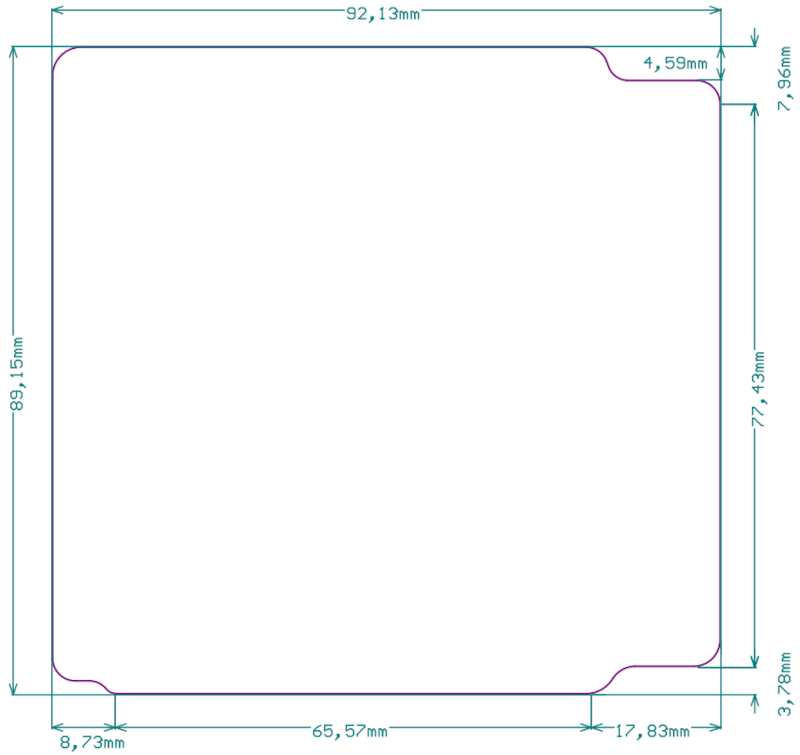
\includegraphics[width=0.7\textwidth]{figures/board-dimensions.png}
        \caption{Board dimensions for the TTC 2.0 module.}
        \label{fig:board-dimensions}
    \end{center}
\end{figure}

\subsection{Layout}

The TTC 2.0 module contains only two layers: top and bottom, as presented in Figures \ref{fig:ttc2-pcb-top} and \ref{fig:ttc2-pcb-bottom}.

\begin{figure}[!ht]
    \begin{center}
        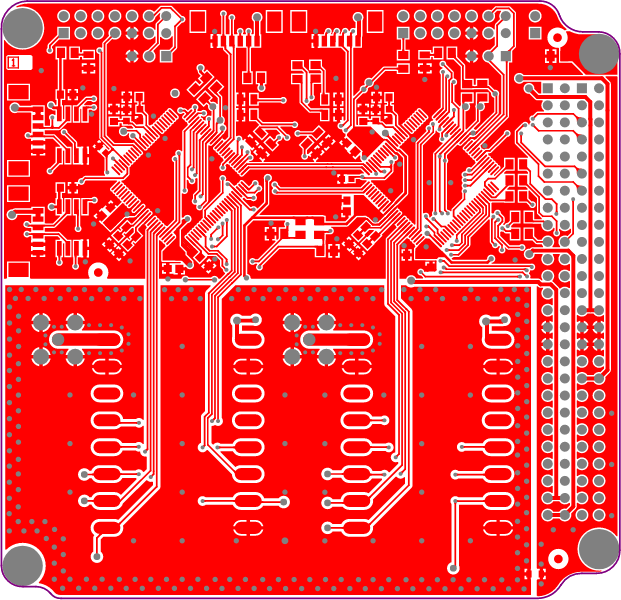
\includegraphics[width=0.7\textwidth]{figures/ttc2-layout-top.png}
        \caption{Top layer of the TTC 2.0 layout.}
        \label{fig:ttc2-layout-top}
    \end{center}
\end{figure}

\begin{figure}[!ht]
    \begin{center}
        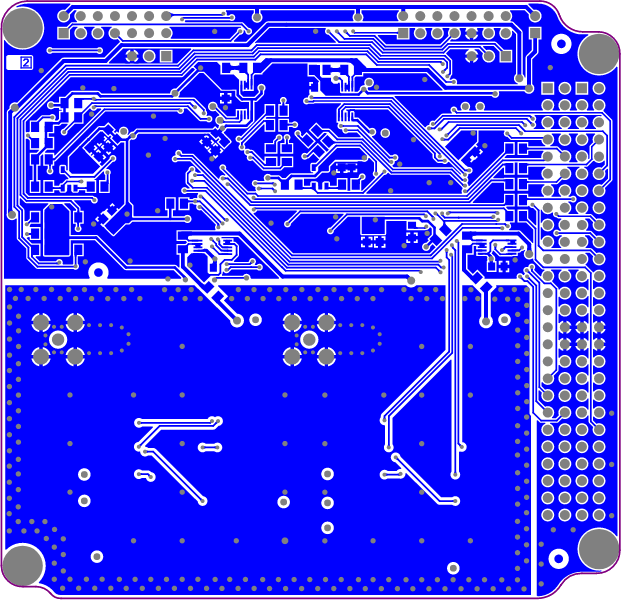
\includegraphics[width=0.7\textwidth]{figures/ttc2-layout-bottom.png}
        \caption{Bottom layer of the TTC 2.0 layout.}
        \label{fig:ttc2-layout-bottom}
    \end{center}
\end{figure}

To design the layout, the Altium Designer\footnote{\href{https://www.altium.com/}{https://www.altium.com/}} software was used.

Simple PCBs with common manufacturing specifications were used to test and develop the module. These PCBs were defined as Engineering Models (EM). The Flight Model (FM, or the boards that fly with the satellite) of the boards have the following manufacturing specifications:

\begin{itemize}
    \item \textbf{PCB specs.}: IPC 6012 Class 3
    \item \textbf{PCB thickness}: 1,6 mm
    \item \textbf{Material}: TG170 FR-4
    \item \textbf{Surface finish}: ENIG
    \item \textbf{Board finish}: Conformal coating application
\end{itemize}

\section{Peripherals}

The TTC 2.0 have some peripherals besides the microcontrollers, like sensors, watchdog timers, and radio modules. These peripherals are better described in this section.

\subsection{Power sensor}

The board has power sensors (model INA226AQDGSRQ1 from Texas Instruments) that use an I$^{2}$C interface to communicate with the microcontroller. There are four of these sensors in the module, one for each microcontroller and one for each radio module. It monitors voltage and current from a given bus through a shunt resistor (with a resistance of $0,1$ $\Omega$). The final measurement is continuous and made by an average of 128 measurements with an interval of 588 $\mu$s between each other.

\subsection{External watchdog timer}

Besides the internal watchdog of the microcontroller, there is also a redundant external one. For that, the TPS3823 IC from Texas Instruments is used. It has an integrated voltage monitor and a watchdog timer, with a timeout of 1600 ms. The boards have two of these ICs, one for each microcontroller.

\subsection{Radio module}

One of the main components of the board is the radio module (NiceRF RF4463F30), which uses an SPI interface to be controlled by the microcontroller. The radio has a dedicated power source of 5V directly from the PC-104 bus. The output power of the RF signal generated by the radio is 30 dBm (1 W). The radio is half-duplex and has an integrated power amplifier and an RF switch, as shown in \autoref{fig:rf4463f30-block-diagram}.

\begin{figure}[!ht]
    \begin{center}
        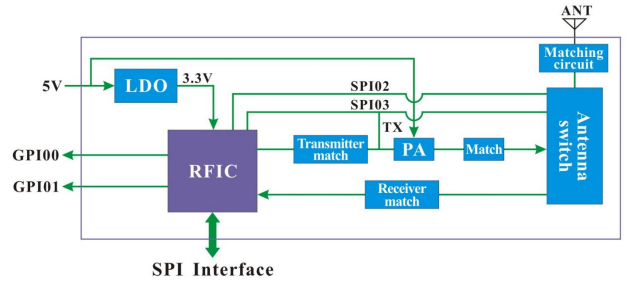
\includegraphics[width=\textwidth]{figures/rf4463f30-block-diagram.png}
        \caption{Block diagram of the RF4463F30 module.}
        \label{fig:rf4463f30-block-diagram}
    \end{center}
\end{figure}